\documentclass[onecolumn]{hipatia}
\usepackage{array}
\newcommand{\PreserveBackslash}[1]{\let\temp=\\#1\let\\=\temp}
\newcolumntype{C}[1]{>{\PreserveBackslash\centering}p{#1}}
\newcolumntype{R}[1]{>{\PreserveBackslash\raggedleft}p{#1}}
\newcolumntype{L}[1]{>{\PreserveBackslash\raggedright}p{#1}}
\begin{document}
\pagestyle{empty}
\pagecolor{olivalight}
\AddToHookNext{shipout/background}
 {%
  \put(0,-\paperheight)
{\begin{tikzpicture}
\meanderbox{8}{13}{0.888}
\end{tikzpicture}}
  \put(420,-125)
{
  
\includegraphics[width=2.2cm]{Hipatiapreto2.png}
}

}

~\\[0.1cm]
\color{cinza}
~\hspace{2.1cm}{\fontsize{26}{32}\selectfont\emph{Revista de Matemática}}
\vspace{0.3cm}
\begin{center}
    {\fontsize{128}{128}\selectfont Hipátia}
\end{center}
\vspace{-0.1cm}
~\hspace{2.1cm}
{\fontsize{18}{18}\selectfont \mesanoedicao}\hfill {\fontsize{18}{18}\selectfont Volume \thevolume, Número \thenumero}\hspace{2cm} 
\vspace{2cm}
\begin{center}


  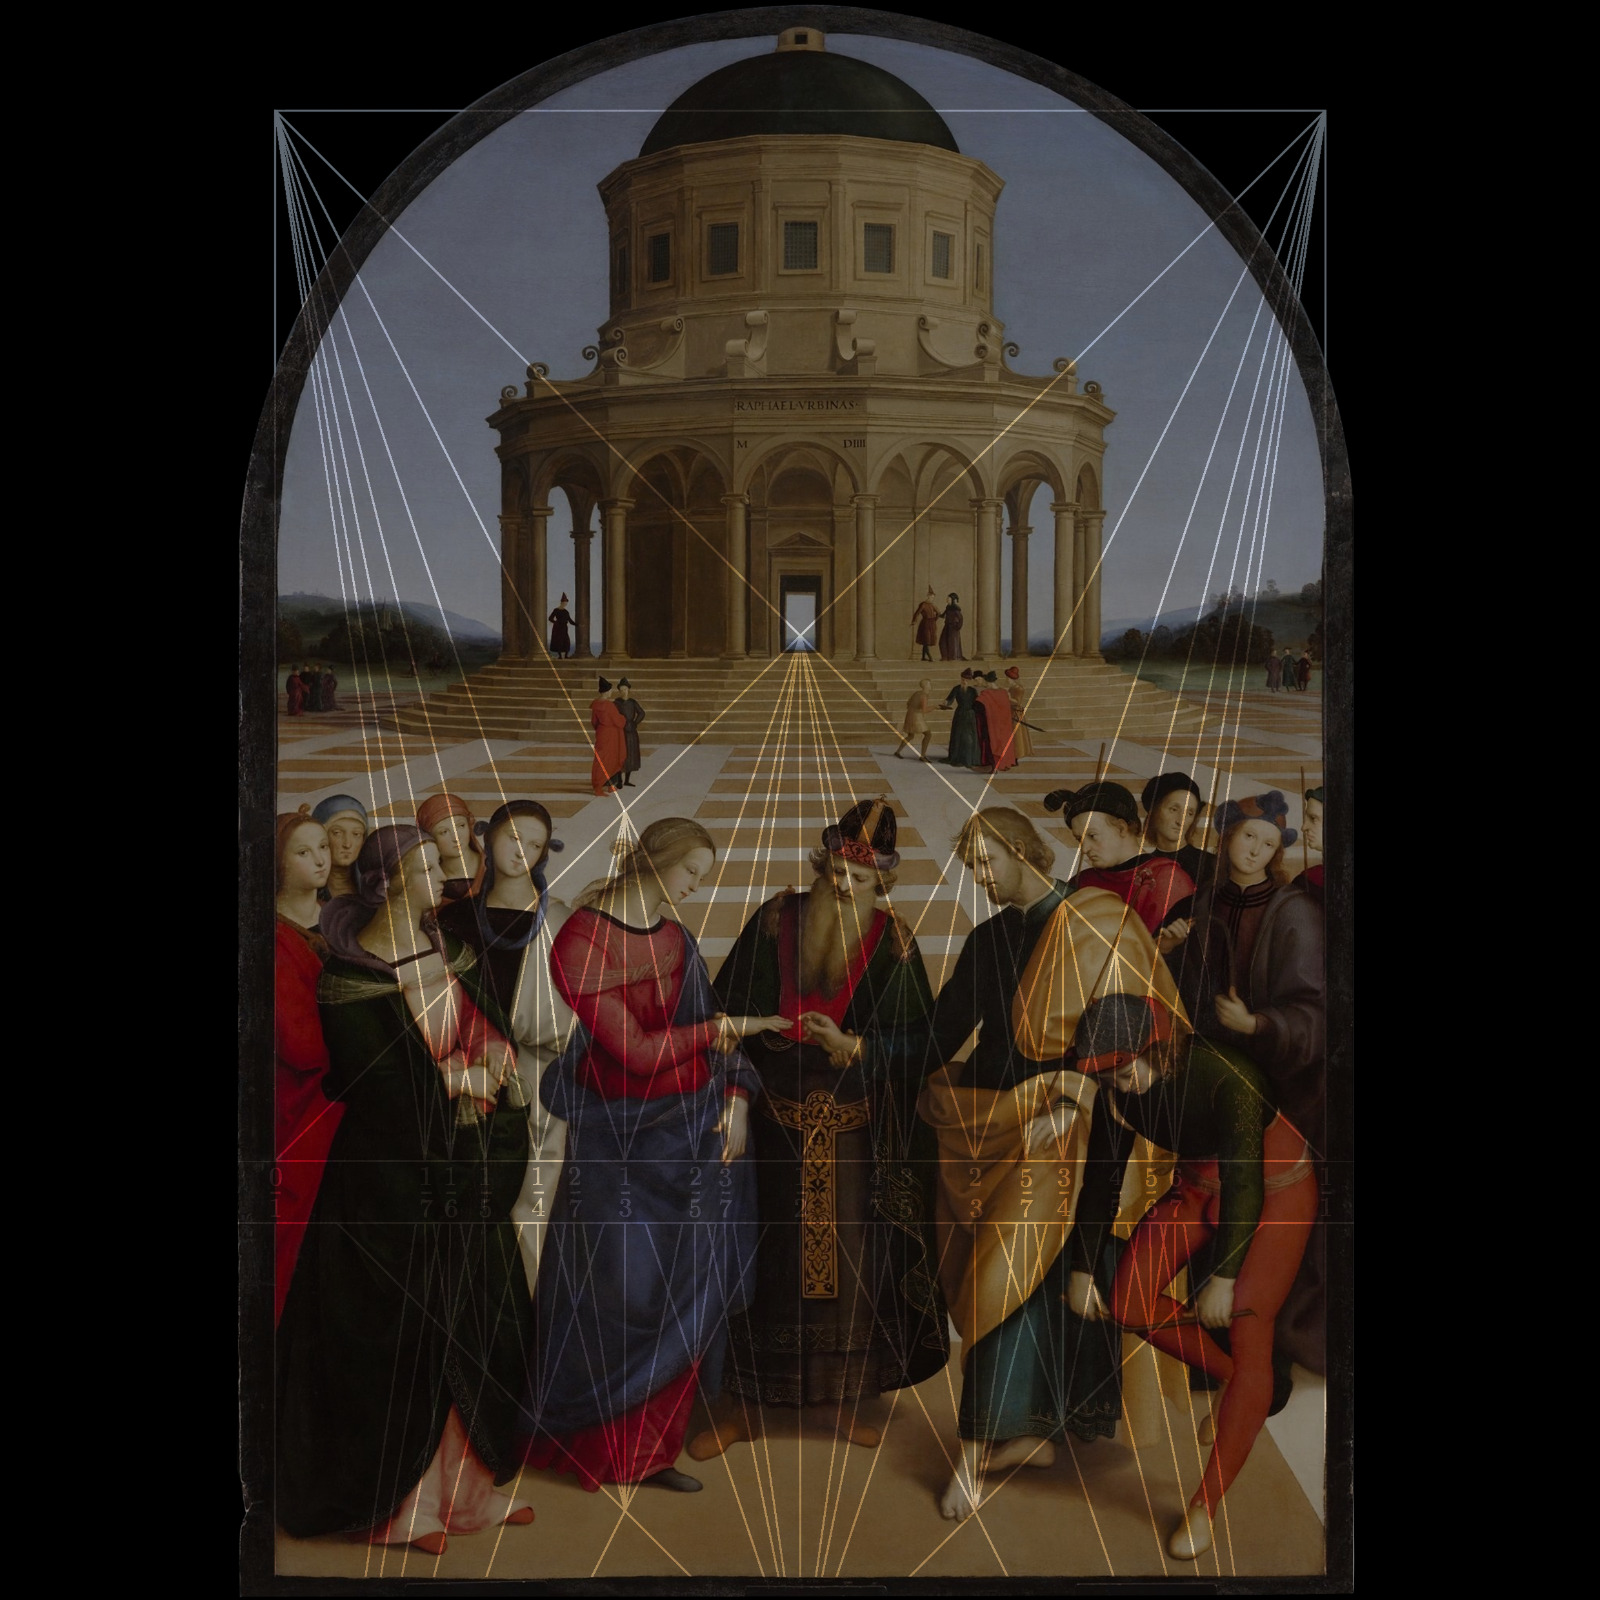
\includegraphics[width=14cm]{Rafael.jpeg}

\vspace{1cm}

{\fontsize{28}{28}\selectfont Rafael --- Casamento da Virgem}
\end{center}
\newpage
~
\newpage
\pagecolor{white}
\begin{center}
  \textbf{UNIVERSIDADE FEDERAL DA BAHIA} \\
  \textbf{Reitor:} Paulo César Miguez de Oliveira\\
\vspace*{0.5cm}
  \textbf{Pró-Reitoria de Extensão Universitária} \\
  \textbf{Pró-Reitor:} Guilherme Bertissolo\\
  \vspace*{0.5cm}  
  \textbf{Instituto de Matemática e Estatística} \\
  \textbf{Diretor:} Kleyber Mota da Cunha\\
  \vspace*{0.5cm}
  \textbf{Departamento de Matemática} \\
  \textbf{Chefe:} Darllan Conceição Pinto\\
\vspace*{2cm}
{\fontsize{23}{23}\selectfont\textit{Revista de Matemática}}\\
\vspace*{0.3cm}
{\fontsize{72}{72}\selectfont Hipátia}\\
\vspace*{0.8cm}
\textbf{Conselho Editorial} \\
André Mandolesi\\
Cristina Lizana\\
Elaís Cidely S. Malheiro\\
Henrique da Costa\\
Márcia Barbosa\\
Nicola Sambonet\\
Roberto Sant'Anna\\
Samuel Feitosa\\
\vspace*{0.2cm}
\textbf{Equipe Técnica} \\
Álisson Conceição\\
Cleber Brito Figueiredo\\
Eldon Barros dos Reis Júnior\\
João Vítor Fonseca \\
José Valdomiro da Silva Neto\\
Taíse Lara de Souza Jorge\\
Yure Carneiro\\
\vspace*{0.3cm}
\textbf{Editor Responsável:} Vinícius Mello  \\

\vspace*{0.3cm}
\textbf{Endereço para Correspondência}\\
Instituto de Matemática e Estatística\\
Av. Milton Santos, s/n, Campus Universitário de Ondina CEP: 40.170-110\\
\texttt{hipatia@ufba.br}\\
%\vspace*{0.5cm}

  
\includegraphics[width=2.7cm]{NEXIME.png}\hspace{2cm}
  \raisebox{1.3cm}{\textbf{ISSN XXXX-XXXX}}\hspace{2cm}
  
\includegraphics[width=2.7cm]{DMAT.png}


\end{center}
\newpage

\pagestyle{empty}
\AddToHookNext{shipout/background}
 {%
  \put(3cm,-\paperheight+7cm)
{\begin{tikzpicture}
\meanderbox{5}{7}{0.888}
\end{tikzpicture}}
}
~\vspace{4cm}
\begin{center}
    \fontsize{32}{32}\selectfont
    \scshape Sinopse
\end{center}
\vspace{1cm}
\begin{center}
    \begin{tabular}{L{10cm}r}
    \textsc{Epístola}     &  \\
    Renovação\dotfill & \epistolapage \\
    \textsc{História}     &  \\
    Uma Descrição da Gênese do& \\
    Método Axiomático \dotfill & \historiapage \\
    \textsc{Técnica}     &  \\
    Caminhando pelas Sequências de Farey\dotfill & \tecnicapage \\
    \textsc{Simpósio}    &  \\
    Eventos do DMAT\dotfill     & \simposiopage\\    
%    \textsc{Didática}    &  \\
%    Solu\c c\~ao de problemas com o uso de & \\
%    grafos e aplica\c c\~oes matriciais\dotfill     & \didaticapage\\
    \textsc{Problema}    &  \\
    O Encontro na Cafeteria & \\
    e Outros Problemas\dotfill     & \problemapage\\        
    \end{tabular}
\end{center}

\end{document}
